\section{Regarding NHST}\label{app:nhst}
Null hypothesis significance testing (NHST, \citealt{fisher1925, neymanpearson1933})
is included here as contextual background rather than as a competing method.
A p-value measures the probability of observing data at least as extreme as those
obtained \emph{assuming the null is true}, $P(\mathrm{data}\mid H_0)$, not the
probability that the null is true given the data, $P(H_0\mid\mathrm{data})$
\citep{cohen1994, wasserstein2016};
consequently, NHST can only reject the null or remain inconclusive; it carries
no mechanism to positively accept it, making it structurally unsuitable for the
precision-and-decisiveness criterion that motivates DPitG.
Understanding its sequential behaviour nevertheless clarifies why the Bayesian
HDI+ROPE framework was developed.

In NHST, at each iteration the experiment stops and $\theta_{\rm null}$ is rejected
whenever the p-value falls below the false positive rate threshold $\alpha_{\rm FPR}$.
Since the decision rule is based solely on this single threshold, data that fail to
trigger rejection yield an inconclusive result rather than evidence in favour of the null.

Using the same fair coin setup ($\theta_{\rm true}=\theta_{\rm null}=0.5$, $N_{\rm min}=30$) described
in the Methods section (\ref{sec:methods}), we apply NHST with $\alpha_{\rm FPR}=0.05$
as the coupled stopping and decision criterion. A reliable sequential method should maintain a
low rejection rate throughout when the null hypothesis is true: as demonstrated in
Section~\ref{sec:fair_coin_large_scale}, the HDI+ROPE algorithm's rejection rate quickly asymptotes near 6\% and
both precision-based methods maintain a zero rejection rate.

Figure~\ref{fig:fair_decisions_nhst} shows the opposite for NHST: the rejection rate
(red solid) grows steadily over time, while the inconclusive proportion (gray dashed)
decreases. To make this trend visible, the simulation is extended to
$N_{\rm max}=30{,}000$ iterations, well beyond the $N_{\rm max}=1{,}500$ used in
the main analysis, since false rejections accumulate slowly and the growing trend
would not be apparent at shorter horizons.

\begin{figure}[h!]
  \centering
  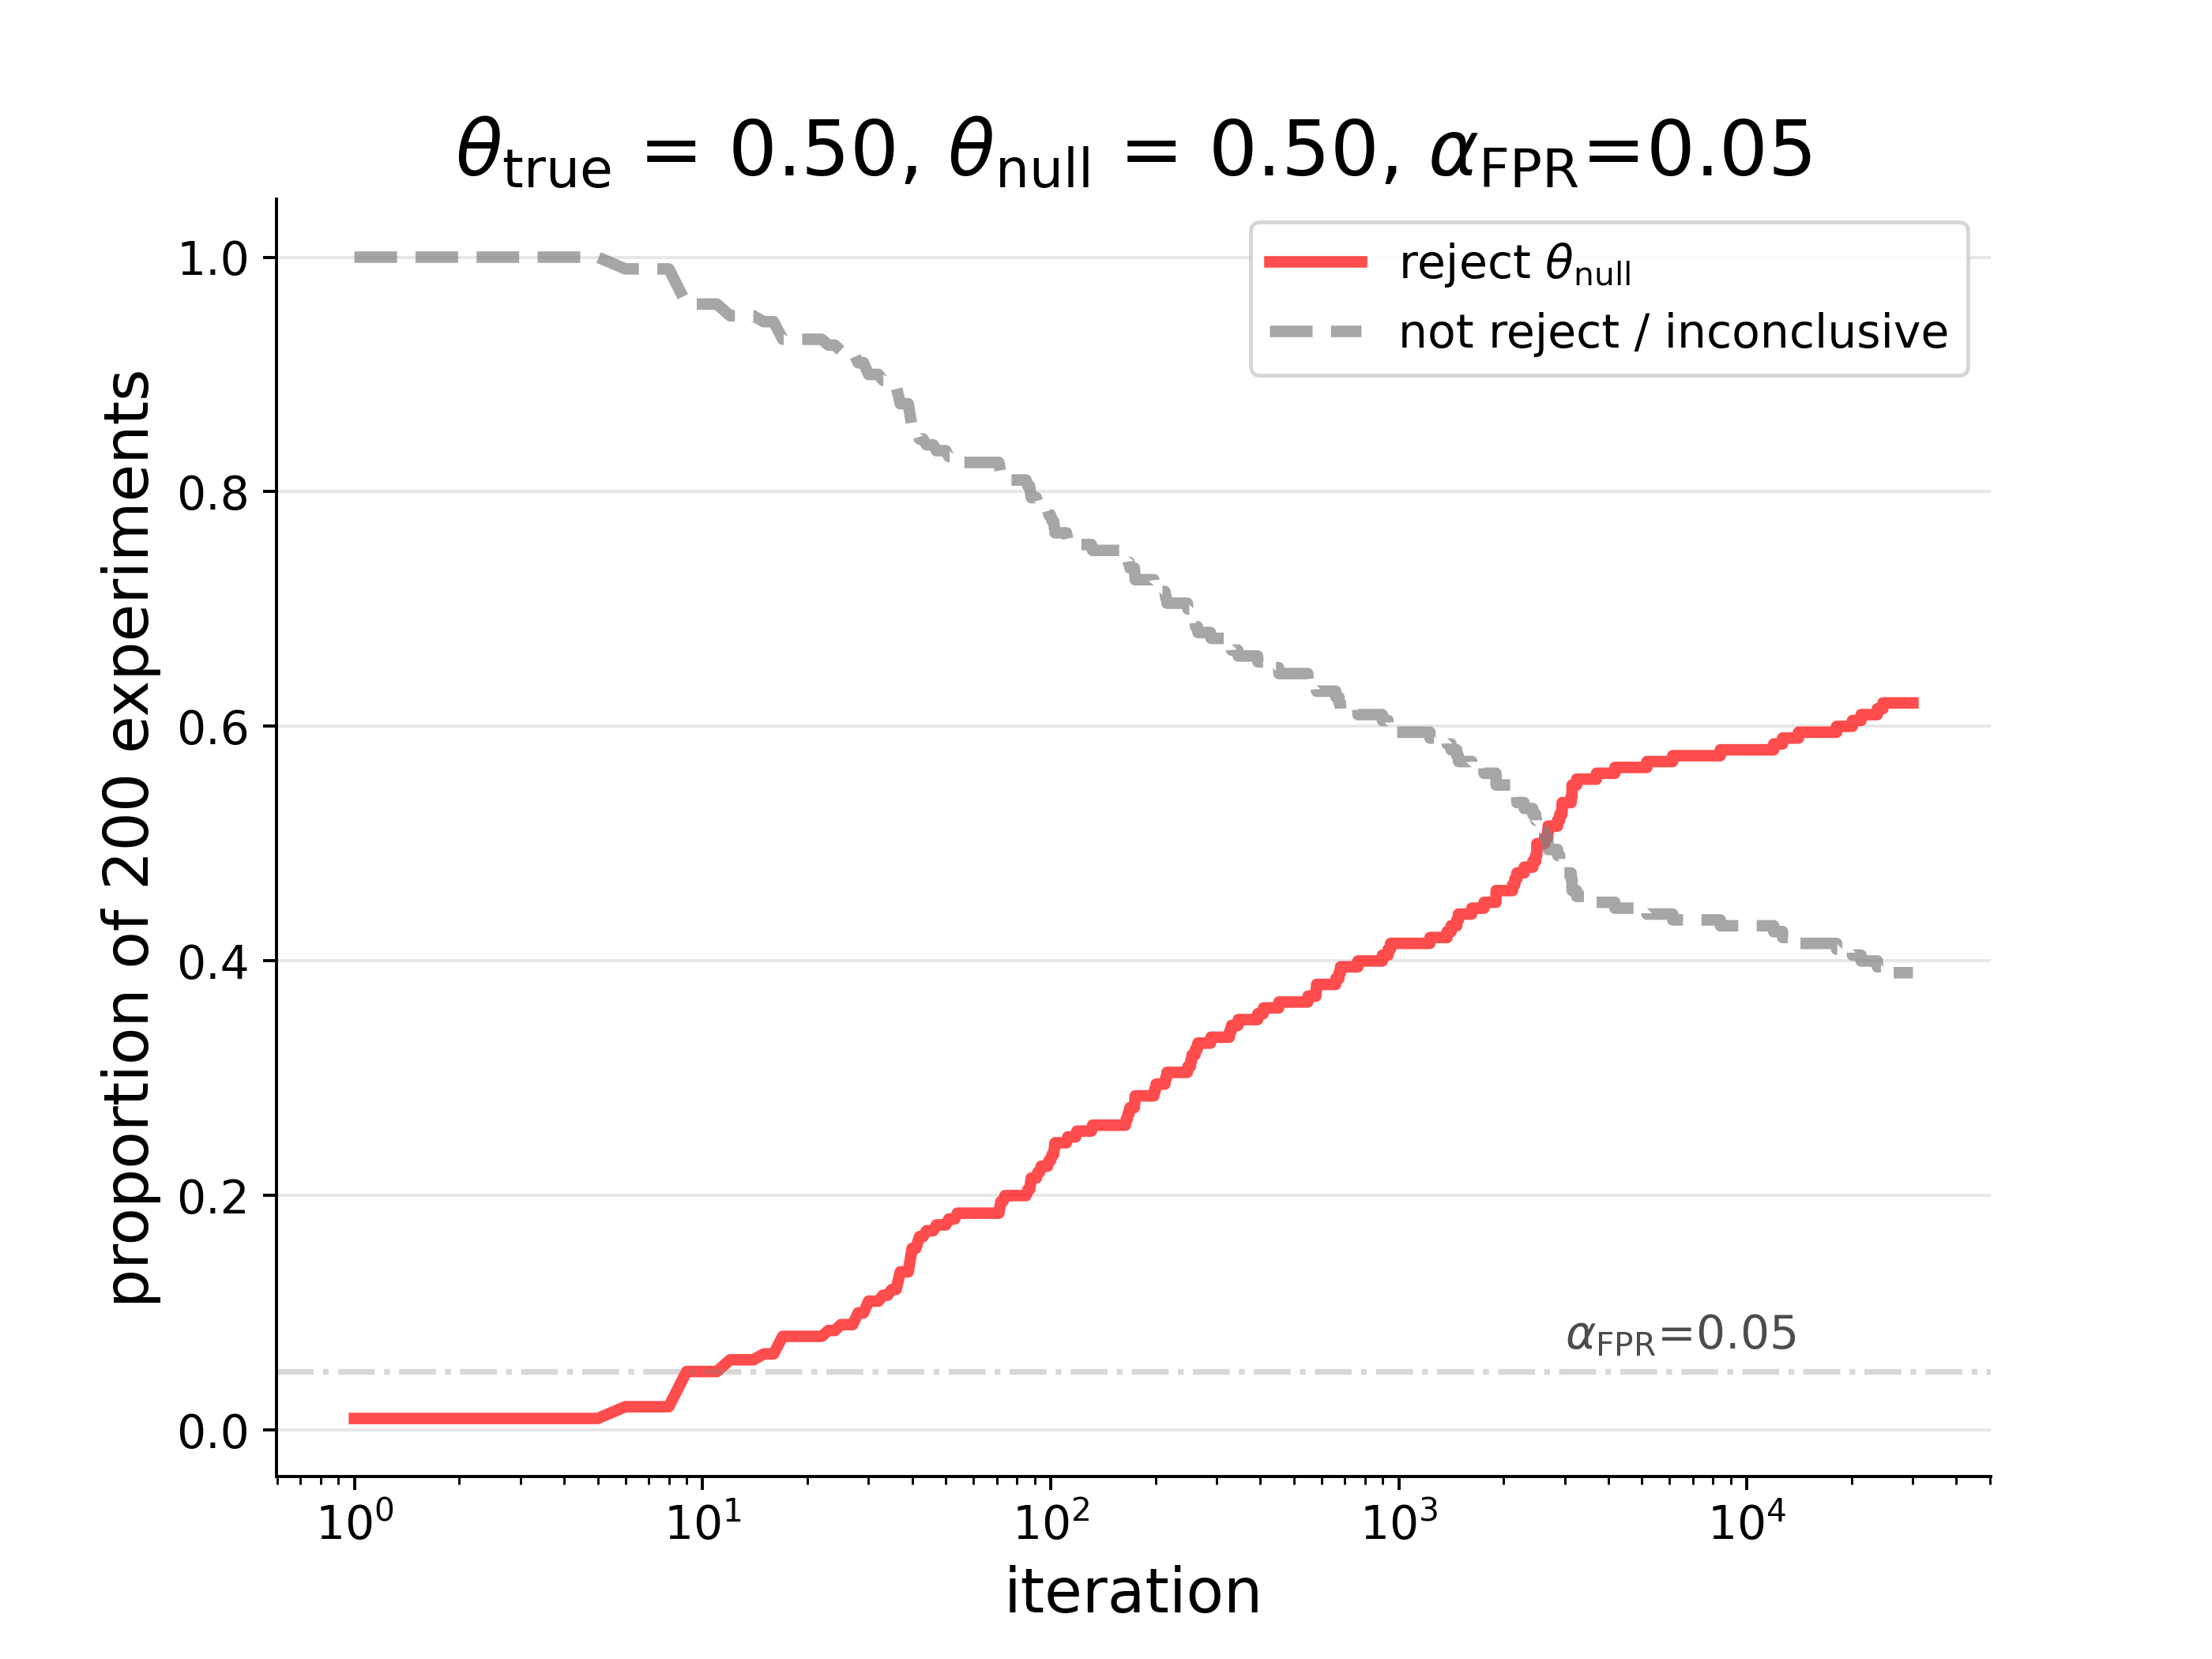
\includegraphics[width=1\textwidth]{faircoin_decision_rates_nhst_dpi350.png}
  \caption{Cumulative decision rates across iterations for $M=200$ fair coin experiments
  ($\theta_{\rm true}=\theta_{\rm null}=0.5$, $\alpha_{\rm FPR}=0.05$,
  $N_{\rm max}=30{,}000$), extending Figure~\ref{fig:fair_decisions} with NHST
  as a fourth panel; it appears in this appendix as NHST lies outside the scope
  of the main analysis.
  At each iteration $N$, the plotted proportions count all experiments that reached
  a decision at or before $N$; their sum is 100\% at every point.
  \textit{Red solid line}: reject $\theta_{\rm null}$.
  \textit{Gray dashed line}: inconclusive.
  The extended horizon ($N_{\rm max}=30{,}000$ vs.\ $1{,}500$ in the main analysis)
  is needed to make the growing false-rejection trend visible; the reduced experiment
  count ($M=200$ vs.\ $5{,}000$) reflects the higher computational cost of evaluating
  p-values relative to HDI-based criteria, which also accounts for the stepped
  appearance of the curves.}
  \label{fig:fair_decisions_nhst}
\end{figure}

As pointed out by \citet{kruschke2015doing}, as evidence accumulates under NHST
the probability of observing a sample extreme enough to trigger rejection grows without
bound, even when the null hypothesis is true. To paraphrase: ``with infinite
peeking, the false positive rate approaches 100\%.'' This is because the stopping
rule is tied directly to the decision rule with no reference to an effect size: the
more data collected, the more likely an extreme sample will appear. Continuously
monitoring the data and applying a fixed p-value threshold therefore leads to an
inflated false-positive (Type~I) error rate, a manifestation of the multiple-testing
problem
\citep{simmons2011}.
Lowering $\alpha_{\rm FPR}$ delays but does not prevent this accumulation: for any
fixed threshold, the false rejection rate still grows without bound as data continue
to be collected.
